\chapter{Progettazione}
\section{Diagramma delle classi }
\begin{center}	
	\vspace{1ex}
	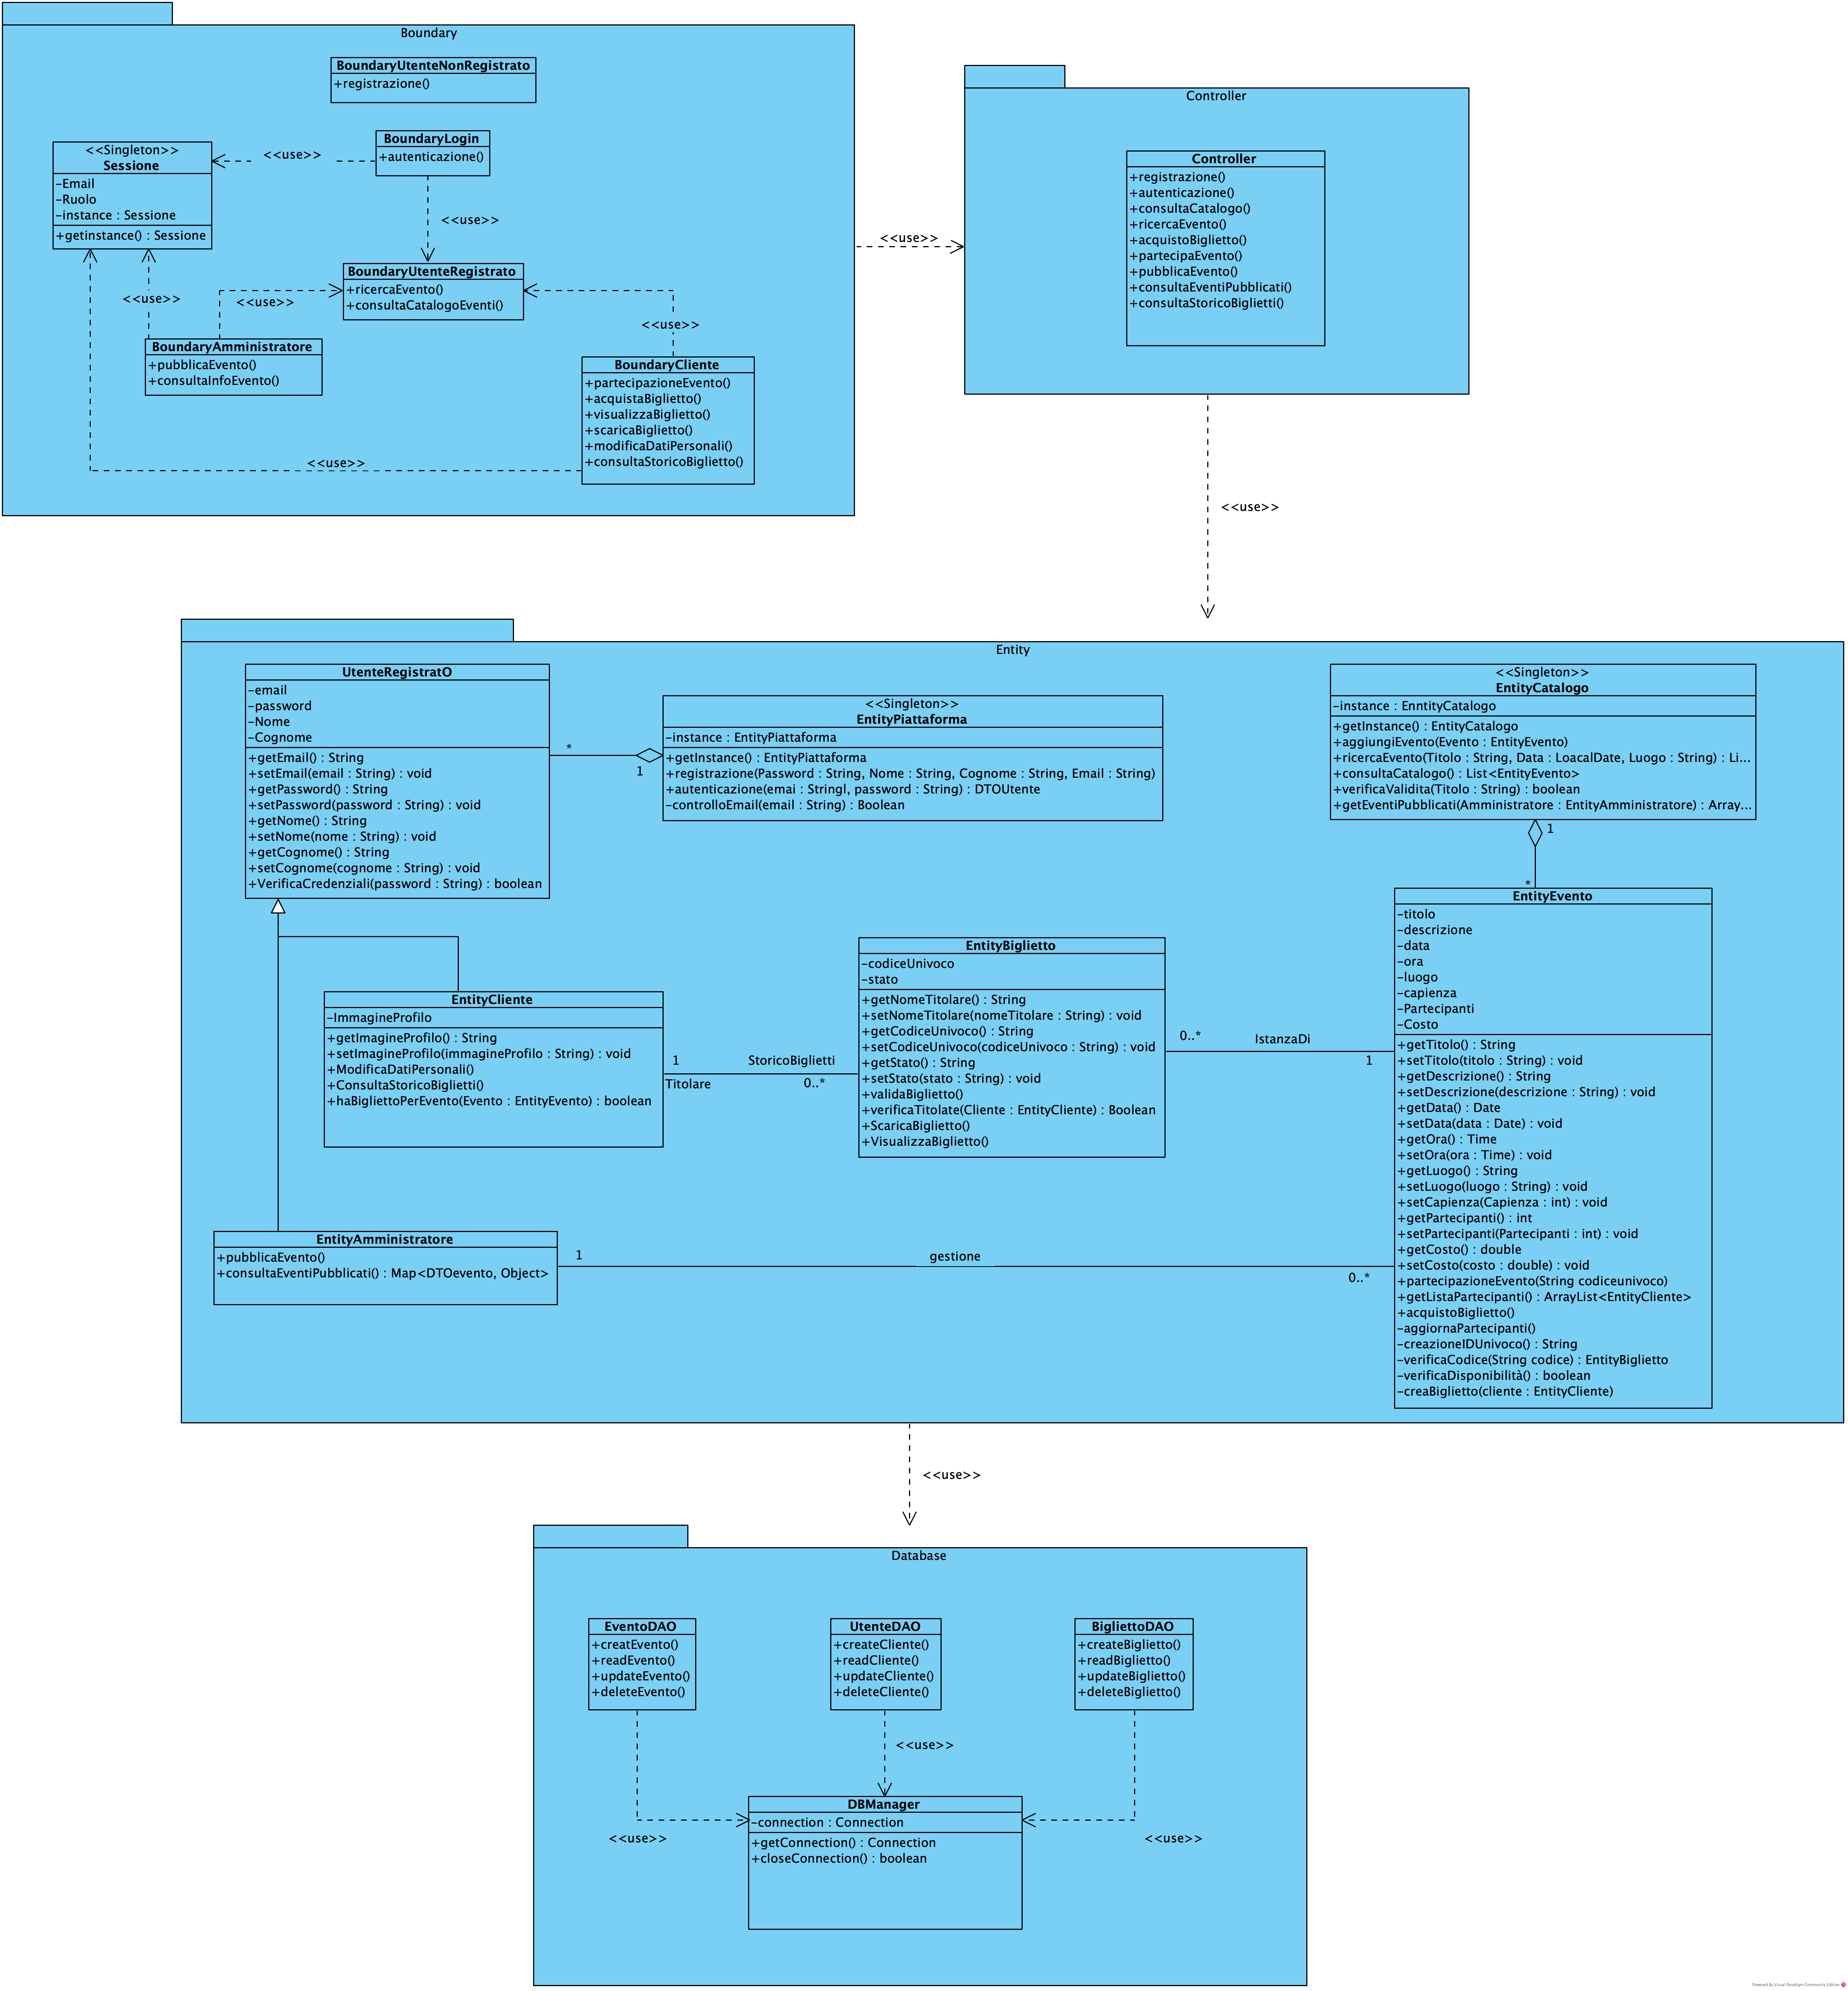
\includegraphics[height=0.9\linewidth]{assets/package/PackageDiagramComplessivo.png}
	\vspace{1ex}
\end{center}
\subsection{Package Entity}
\begin{center}	
	\vspace{1ex}
	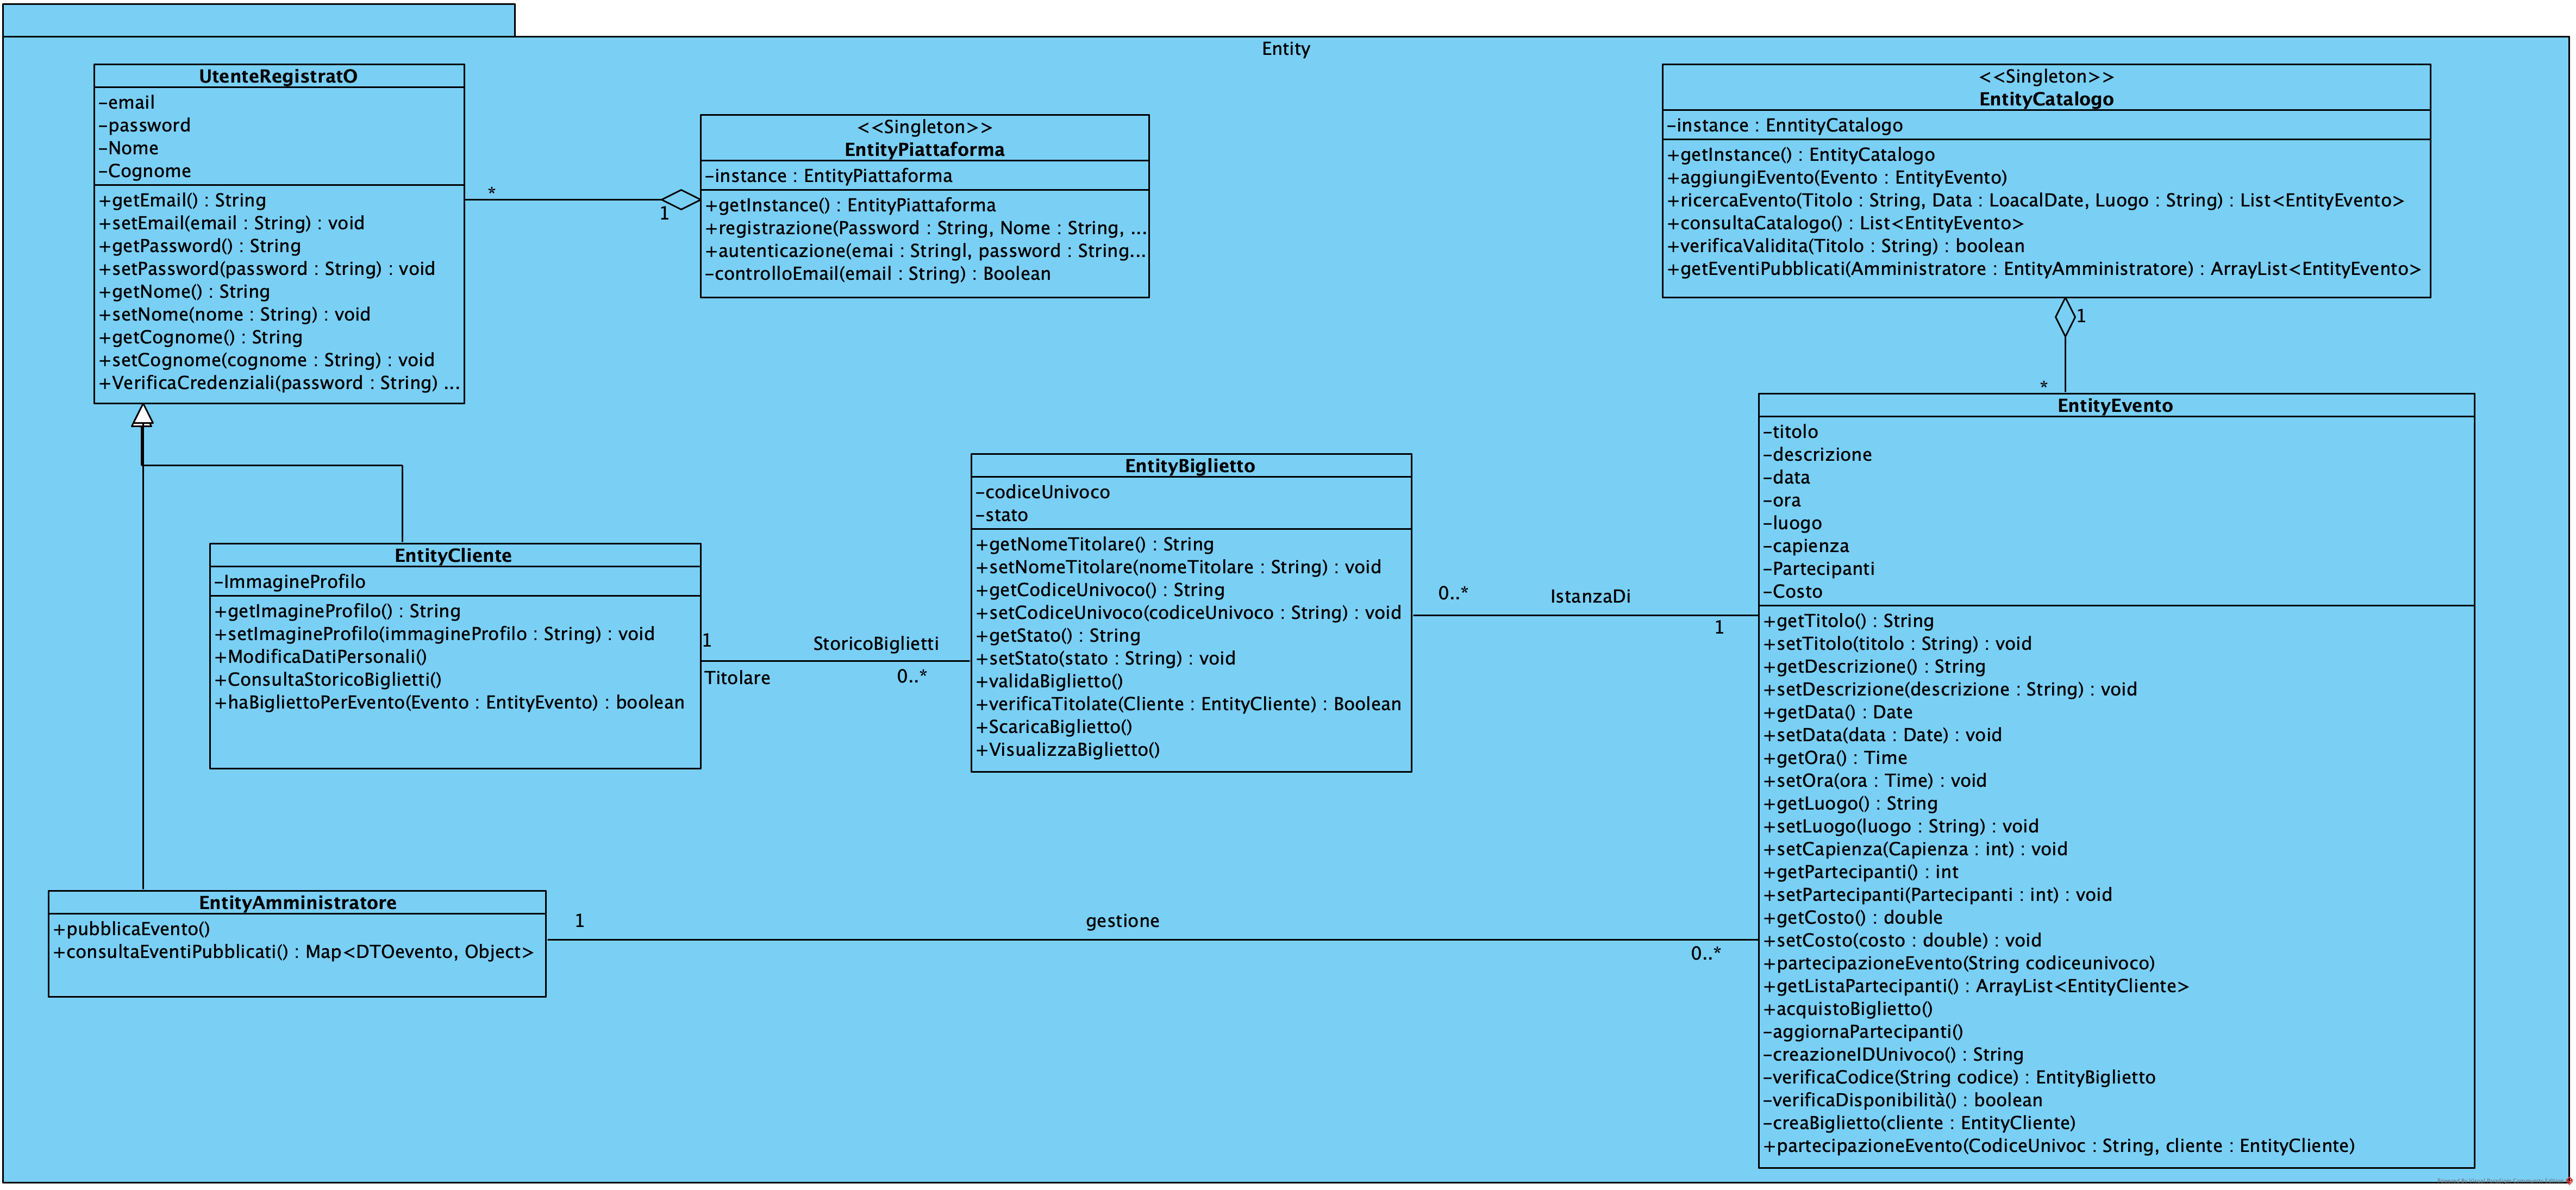
\includegraphics[height=0.38\linewidth]{assets/package/PackageEntity.png}
	\vspace{1ex}
\end{center}
\subsection{Package Boundary}
\begin{center}	
	\vspace{1ex}
	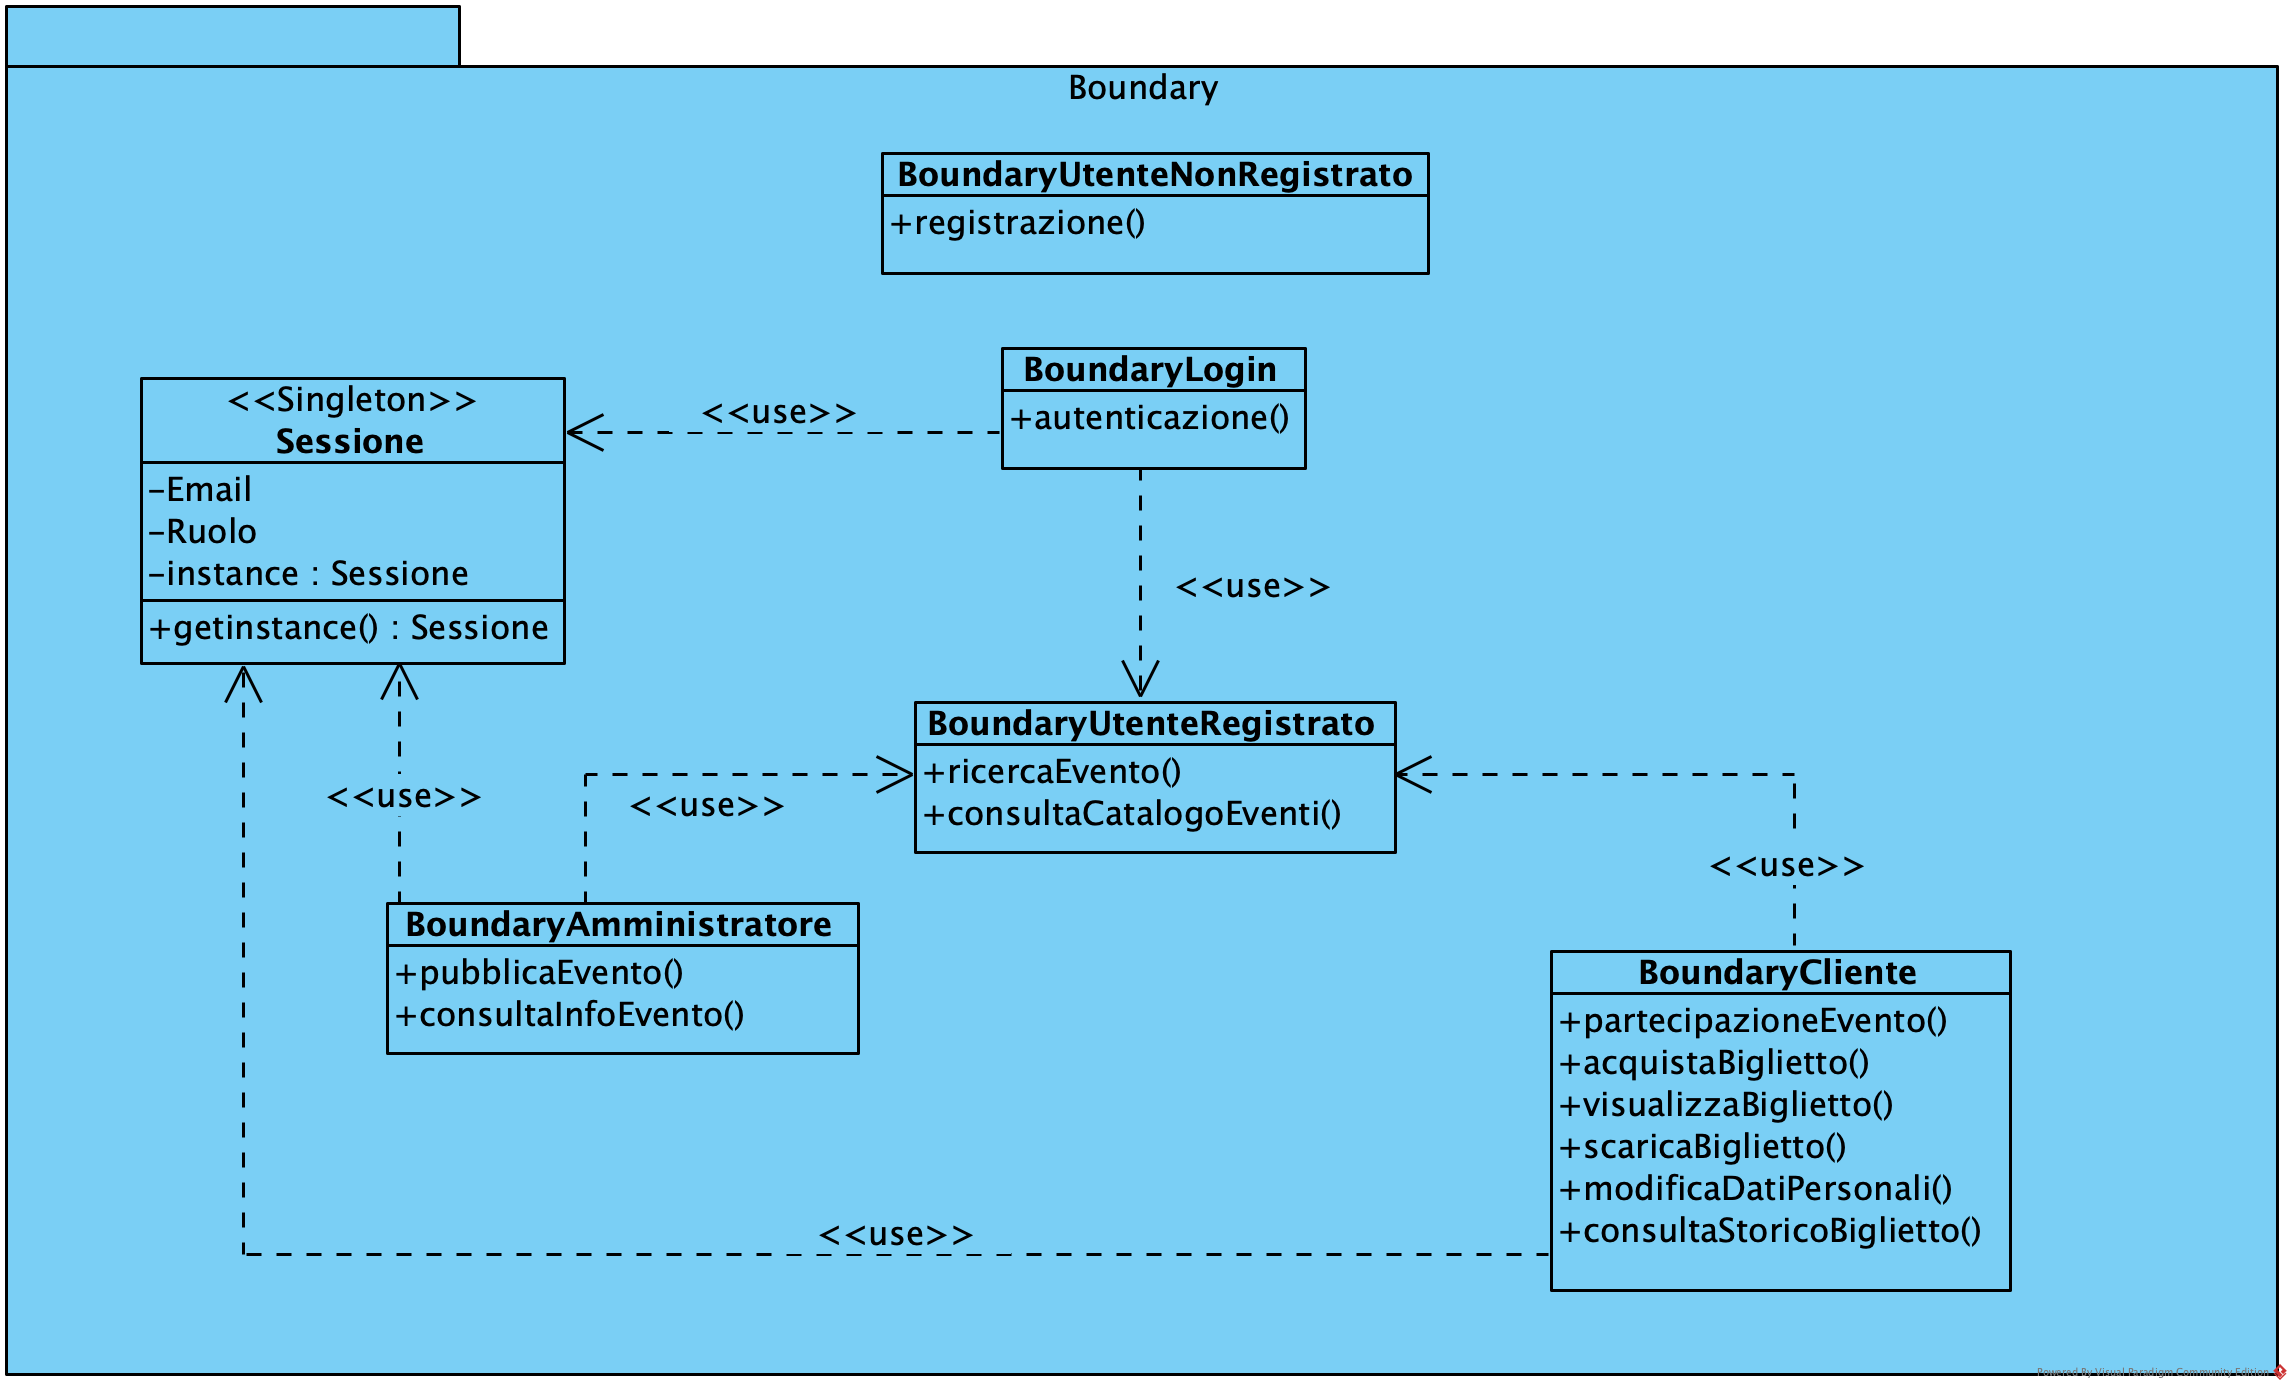
\includegraphics[height=0.38\linewidth]{assets/package/PackageBoundary.png}
	\vspace{1ex}
\end{center}
\subsection{Package Controller}
\begin{center}	
	\vspace{1ex}
	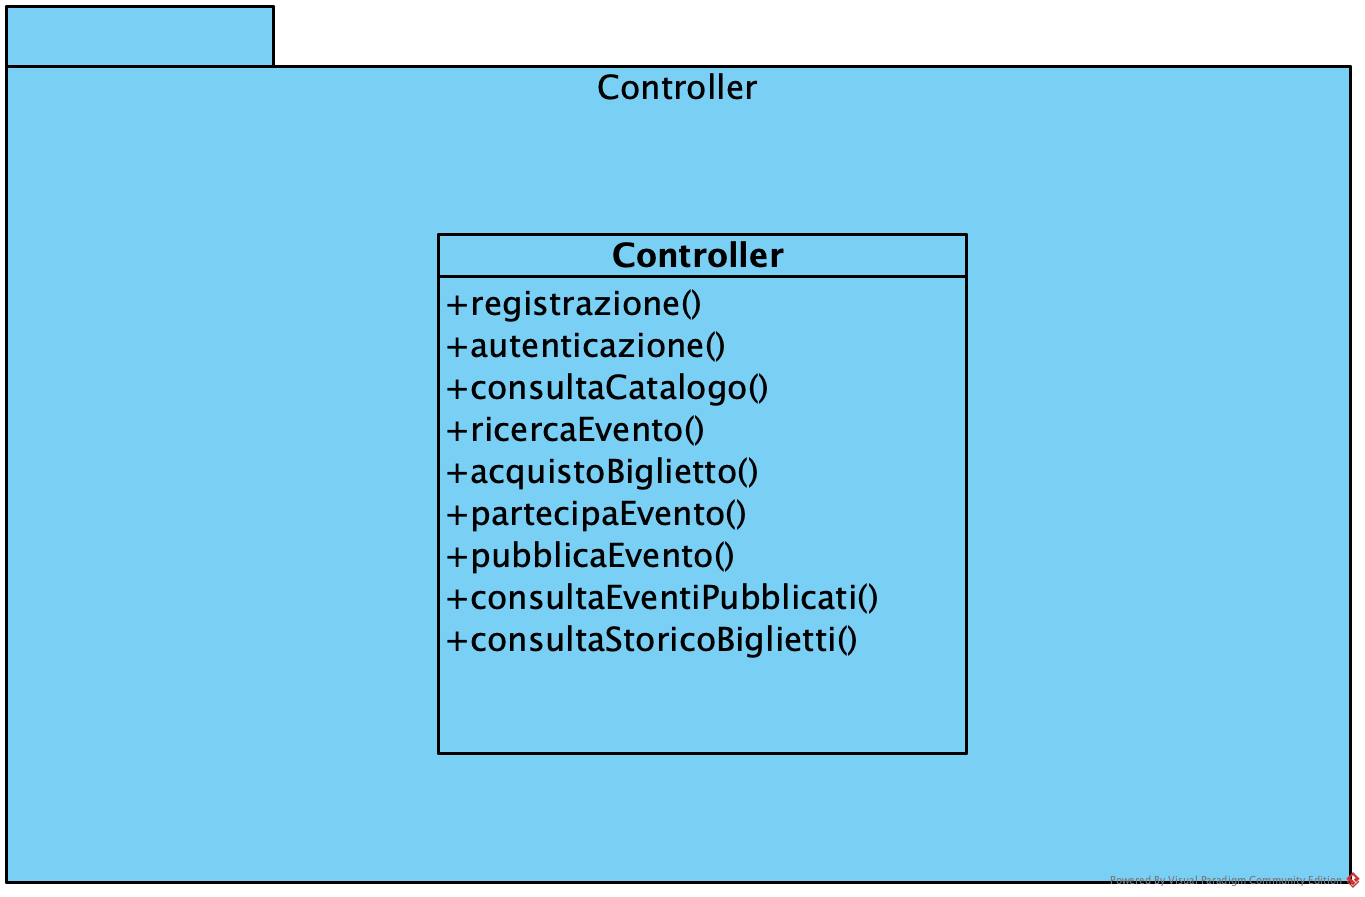
\includegraphics[height=0.38\linewidth]{assets/package/PackageController.png}
	\vspace{1ex}
\end{center}
\subsection{Package Database}

\begin{center}	
	\vspace{1ex}
	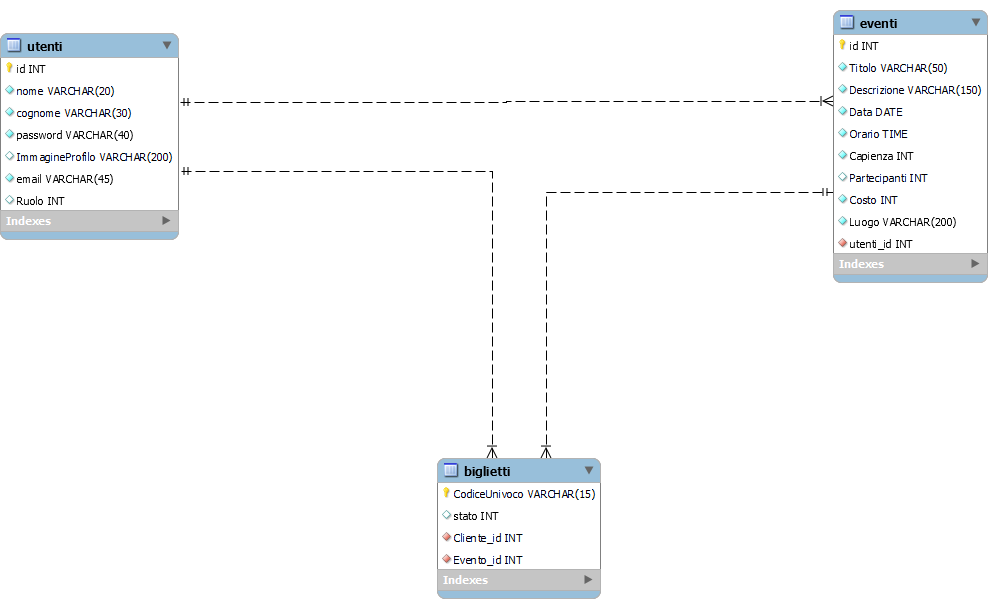
\includegraphics[height=0.38\linewidth]{assets/package/erdiagram.png}
	\vspace{1ex}
\end{center}

\begin{center}	
	\vspace{1ex}
	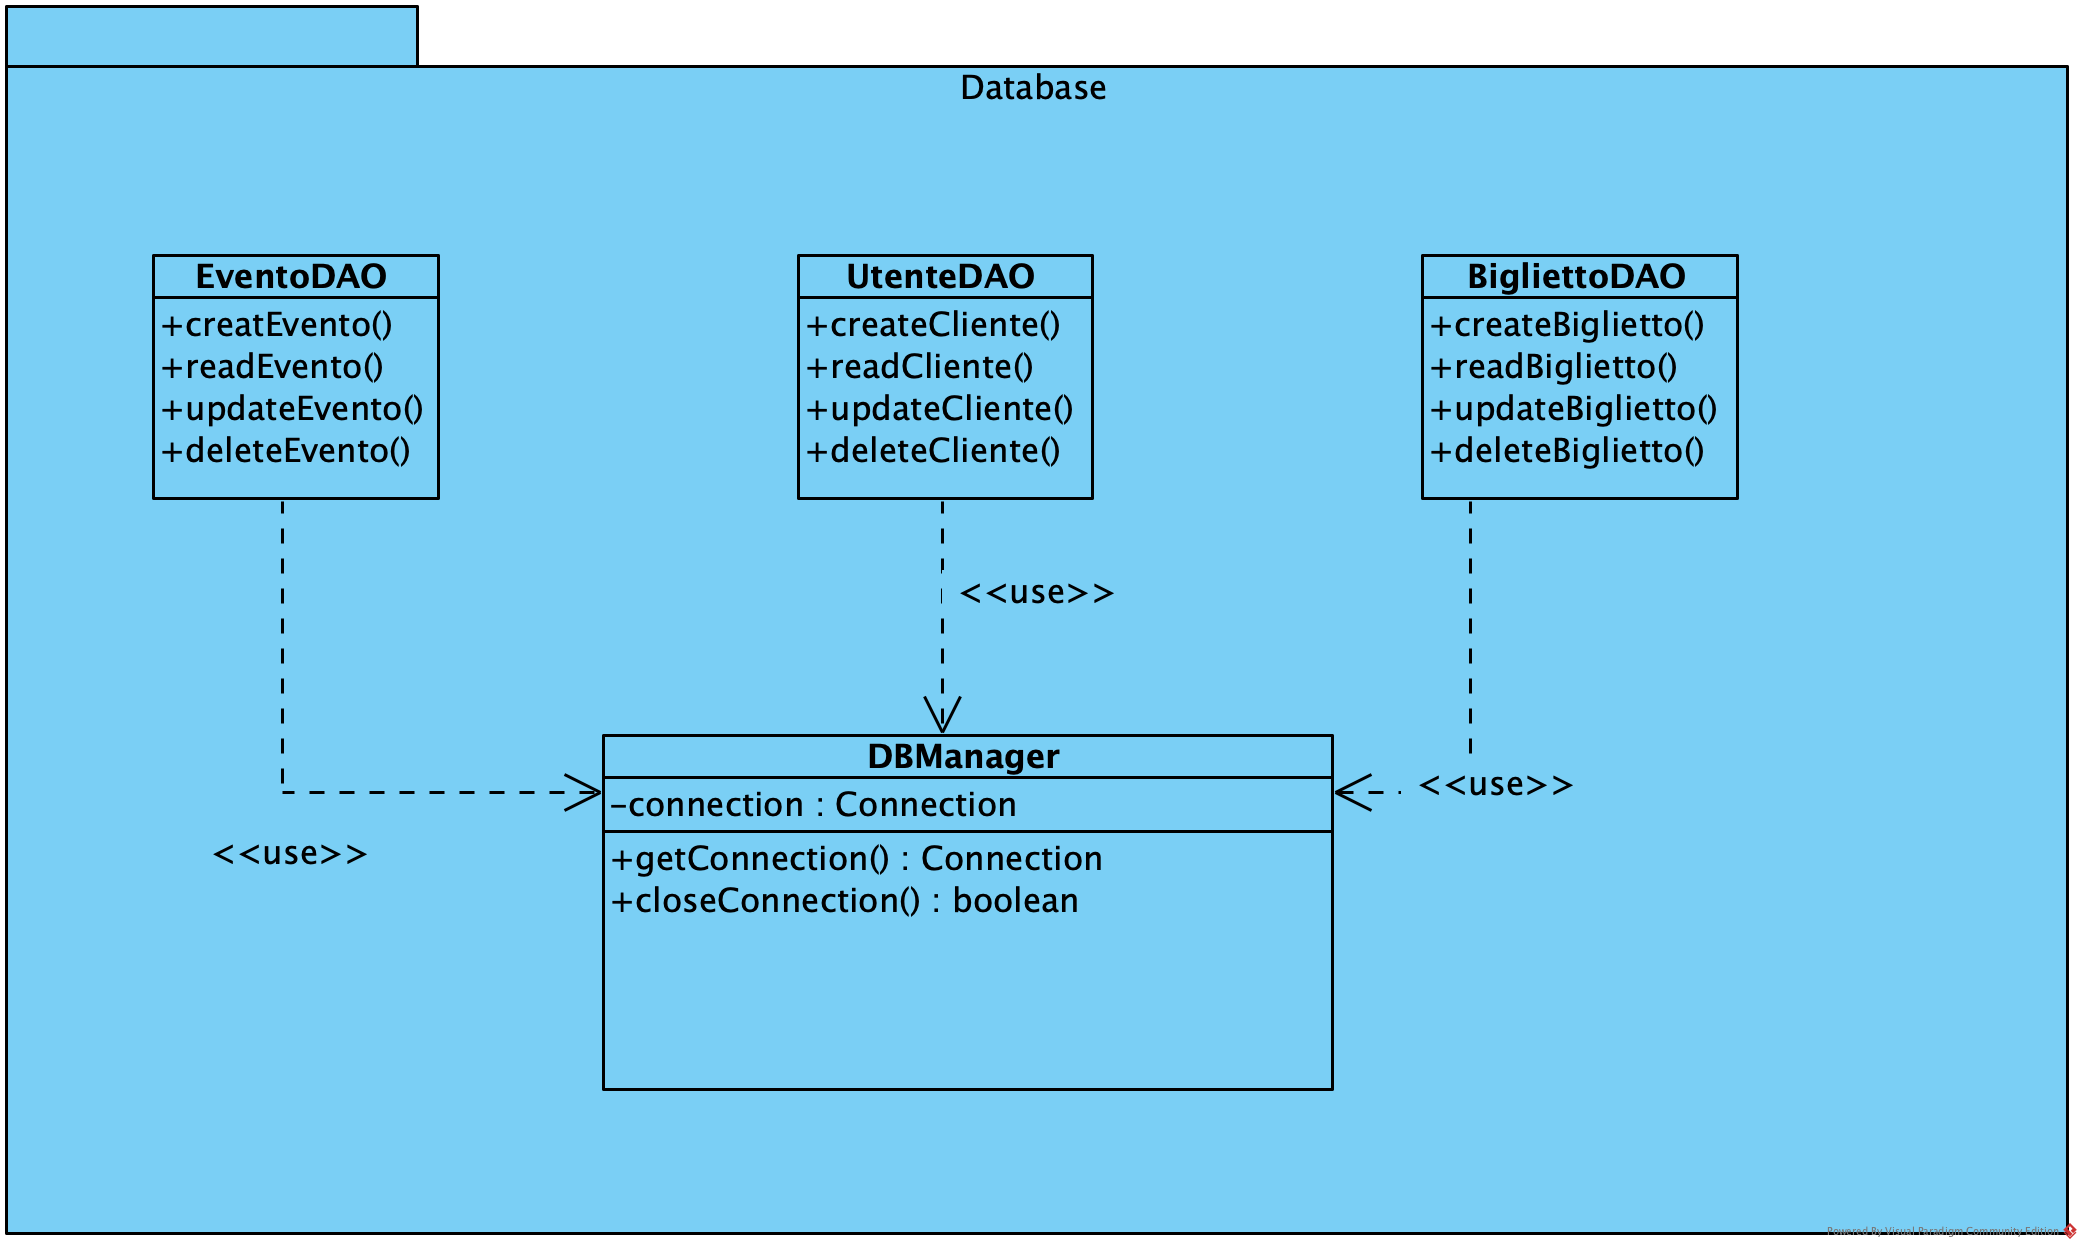
\includegraphics[height=0.38\linewidth]{assets/package/PackageDatabase.png}
	\vspace{1ex}
\end{center}

Il modello E-R riportato rappresenta le principali entità e relazioni del sistema, progettato utilizzando MySQL Workbench.

In fase di progettazione si è scelto di rappresentare tutte e due i ruoli degli utenti all'interno di un'unica tabella denominata `Utente`. All'interno di questa tabella è stato inserito un attributo aggiuntivo, chiamato `Ruolo`, che consente di discriminare i due tipi di utente.

\section{Diagrammi di sequenza}
I seguenti sono i Sequence Diagram relativi alla fase di progettazione. Poiché si tratta di immagini molto dettagliate, si consiglia la visione tramite il file .vpp del progetto

\subsection*{ConsultaEventiPubblicati}
\begin{figure}[H]
\centering
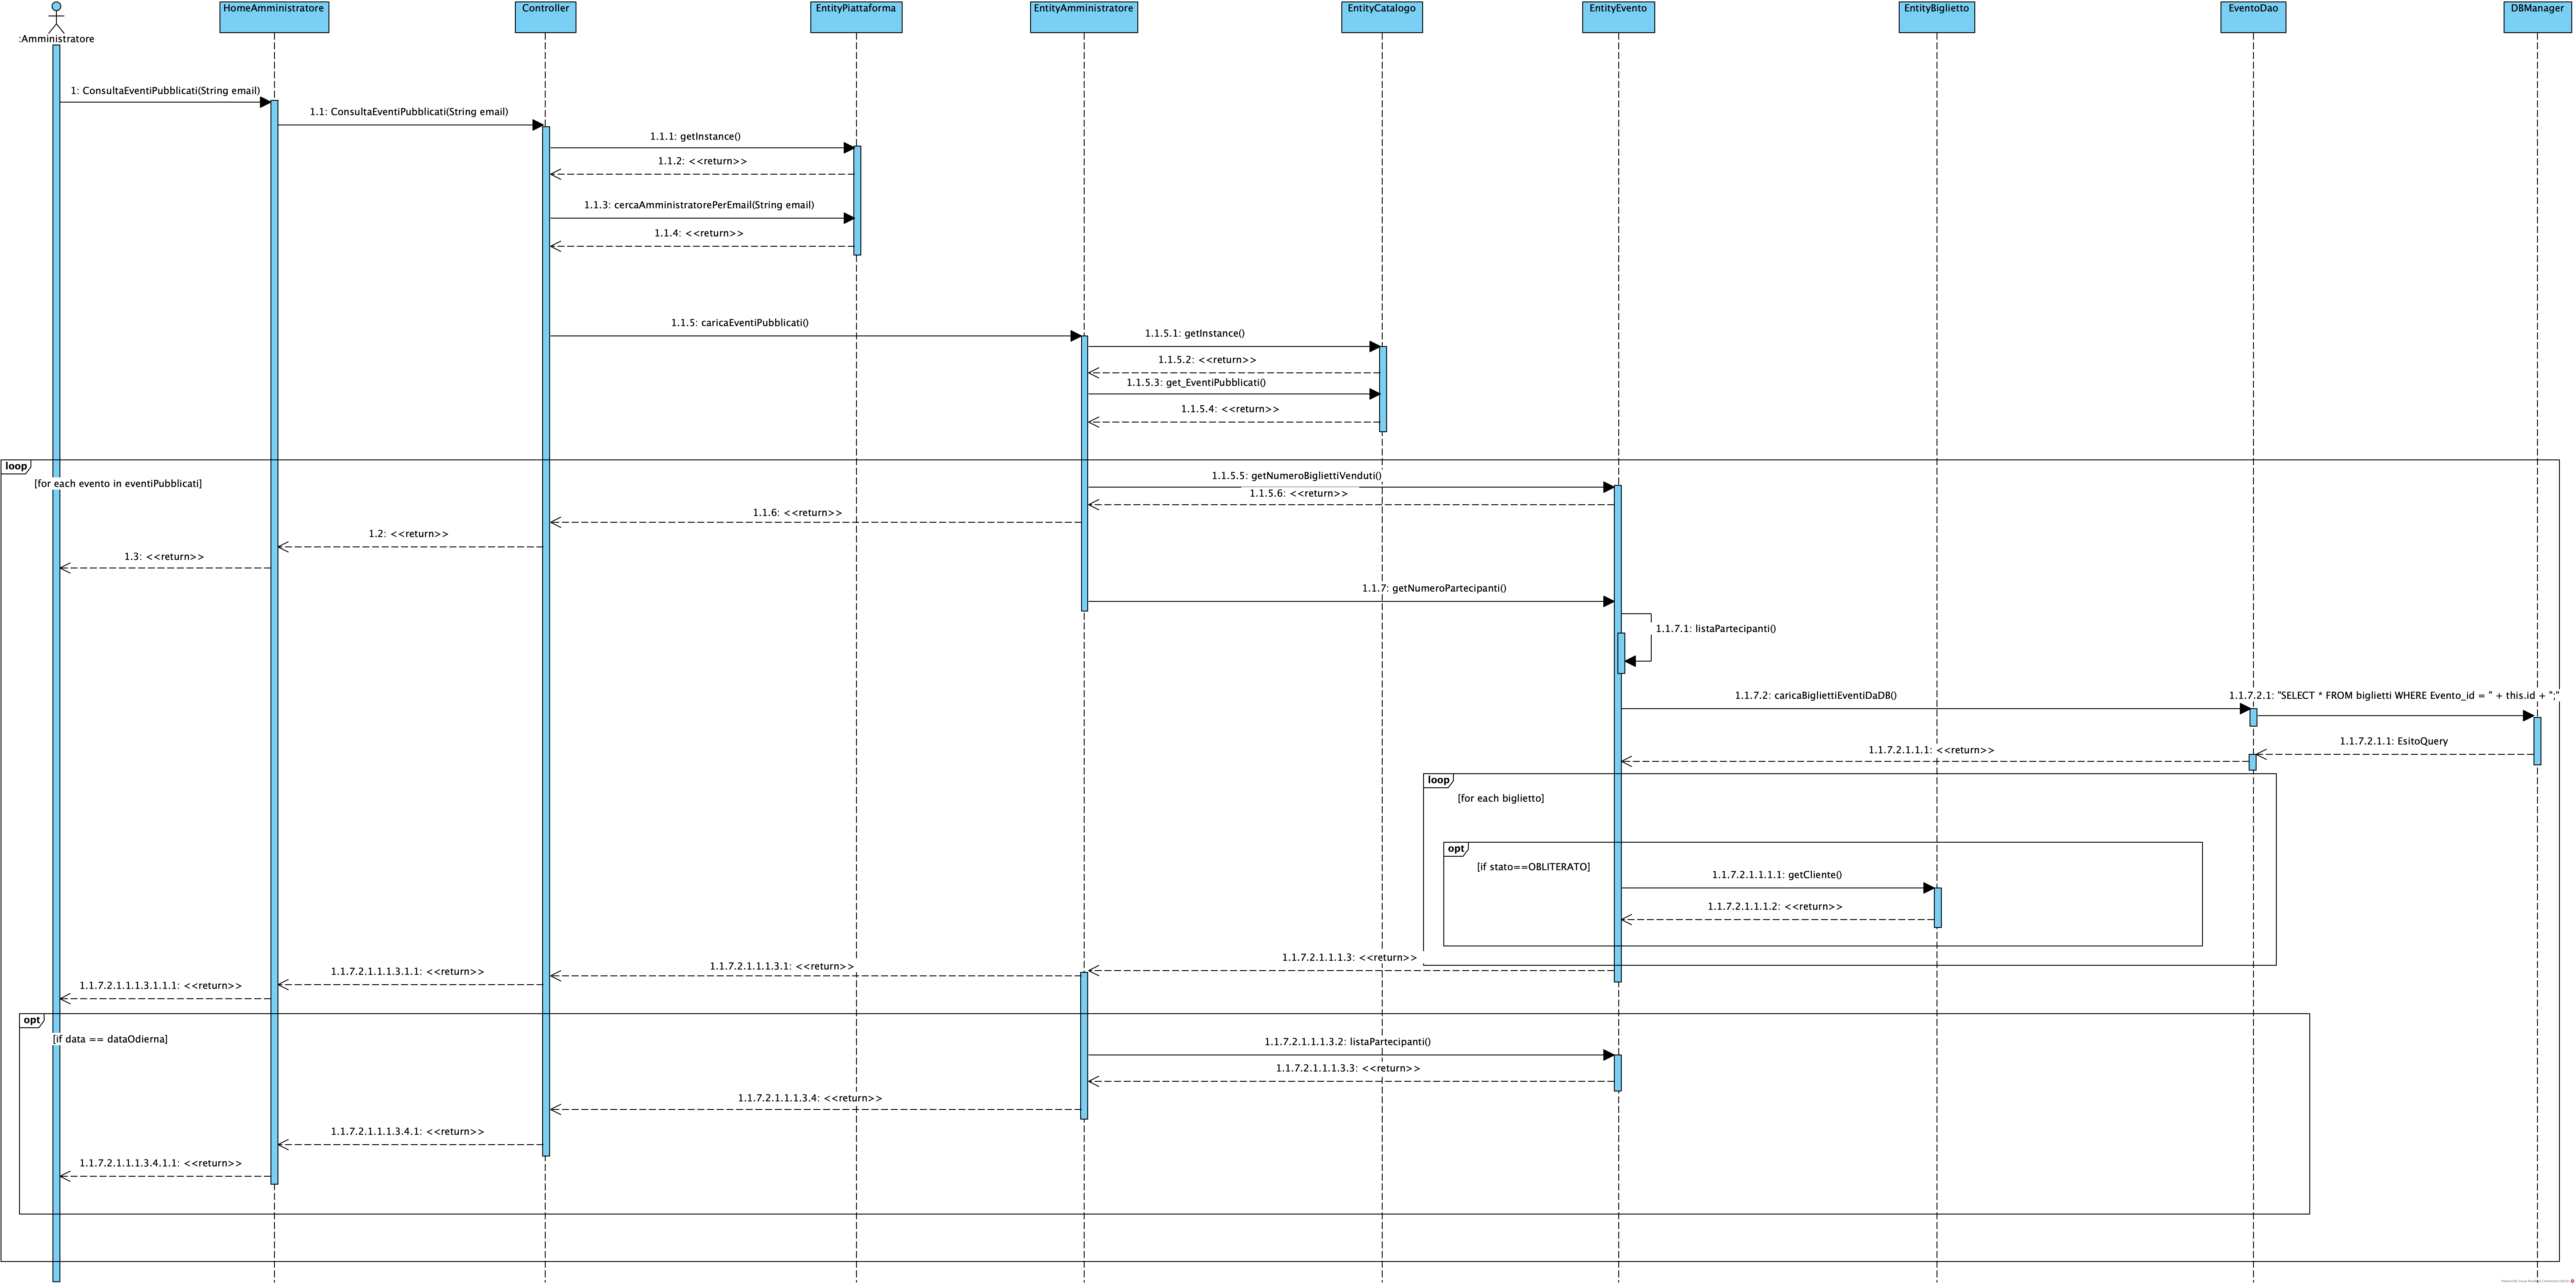
\includegraphics[width=\linewidth]{assets/SDProgettazione/ConsultaEventiPubblicatiProgettazione.png}
\caption{Sequence Diagram avanzato dello scenario \textit{ConsultaEventiPubblicati}}
\end{figure}

\subsection*{AcquistoBiglietti}
\begin{figure}[H]
\centering
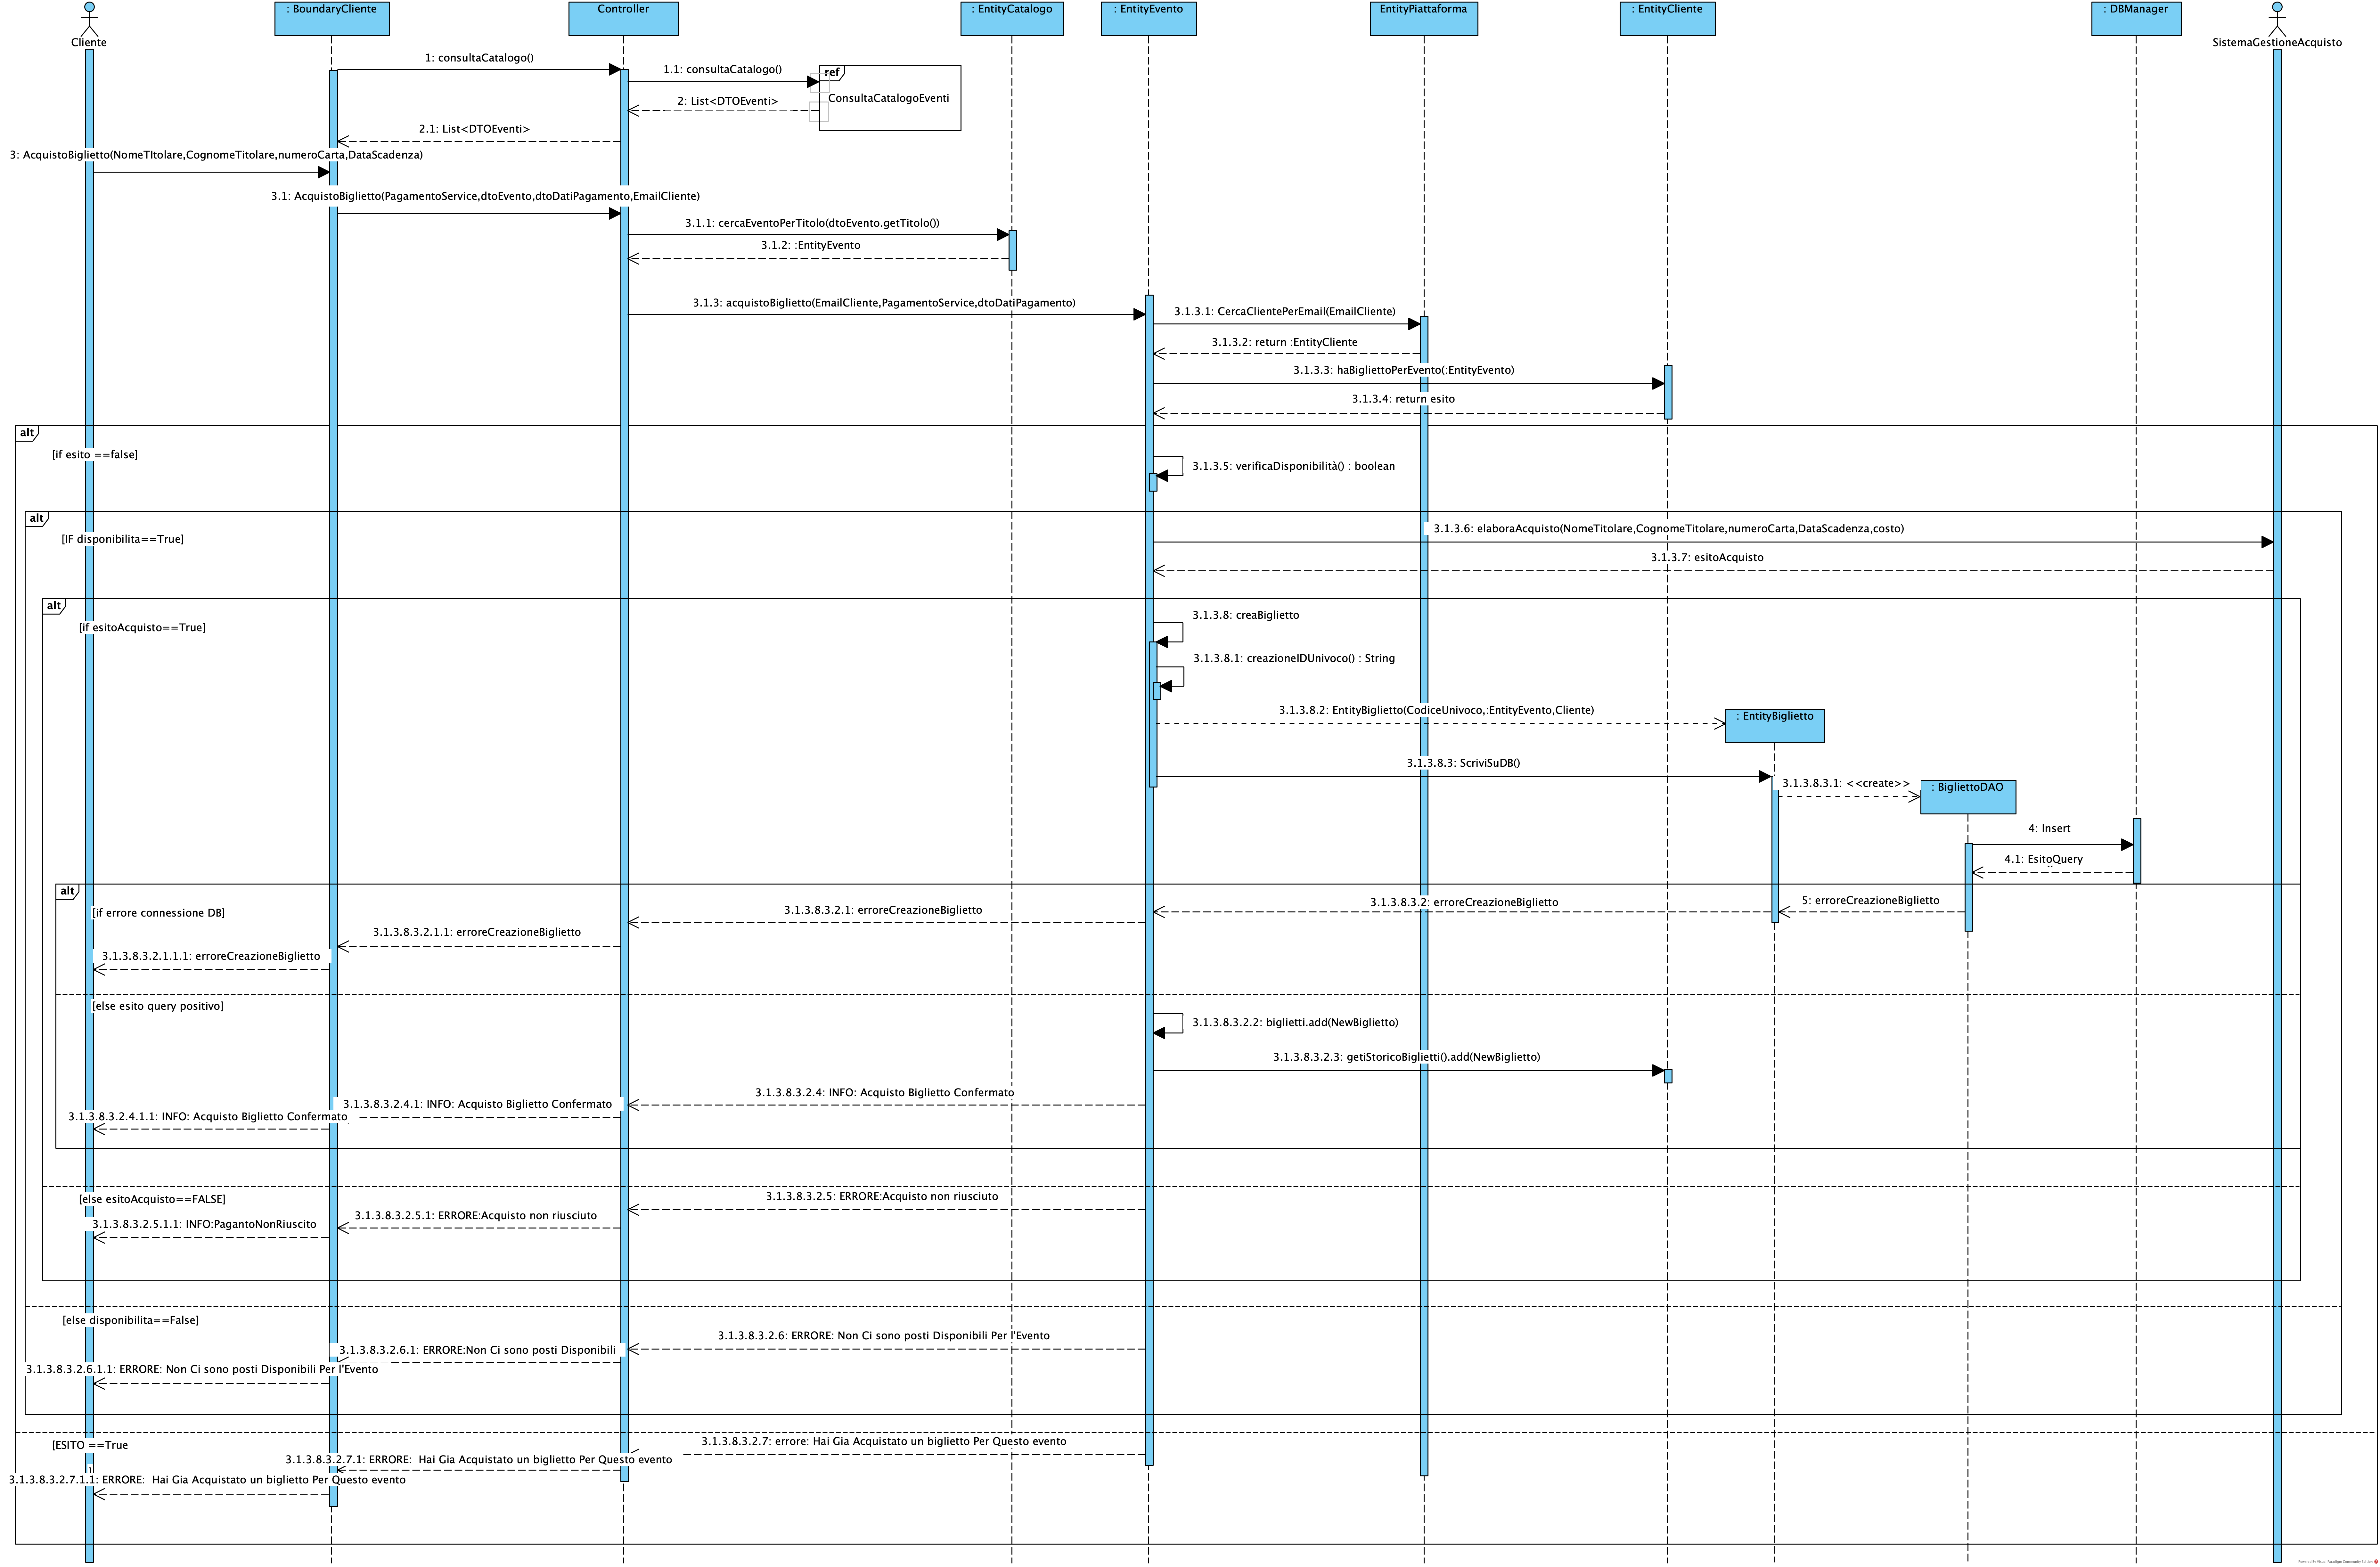
\includegraphics[width=\linewidth]{assets/SDProgettazione/AcquistoBigliettiProgettazione.png}
\caption{Sequence Diagram avanzato dello scenario \textit{AcquistoBiglietti}}
\end{figure}

\subsection*{PartecipazioneEvento}
\begin{figure}[H]
\centering
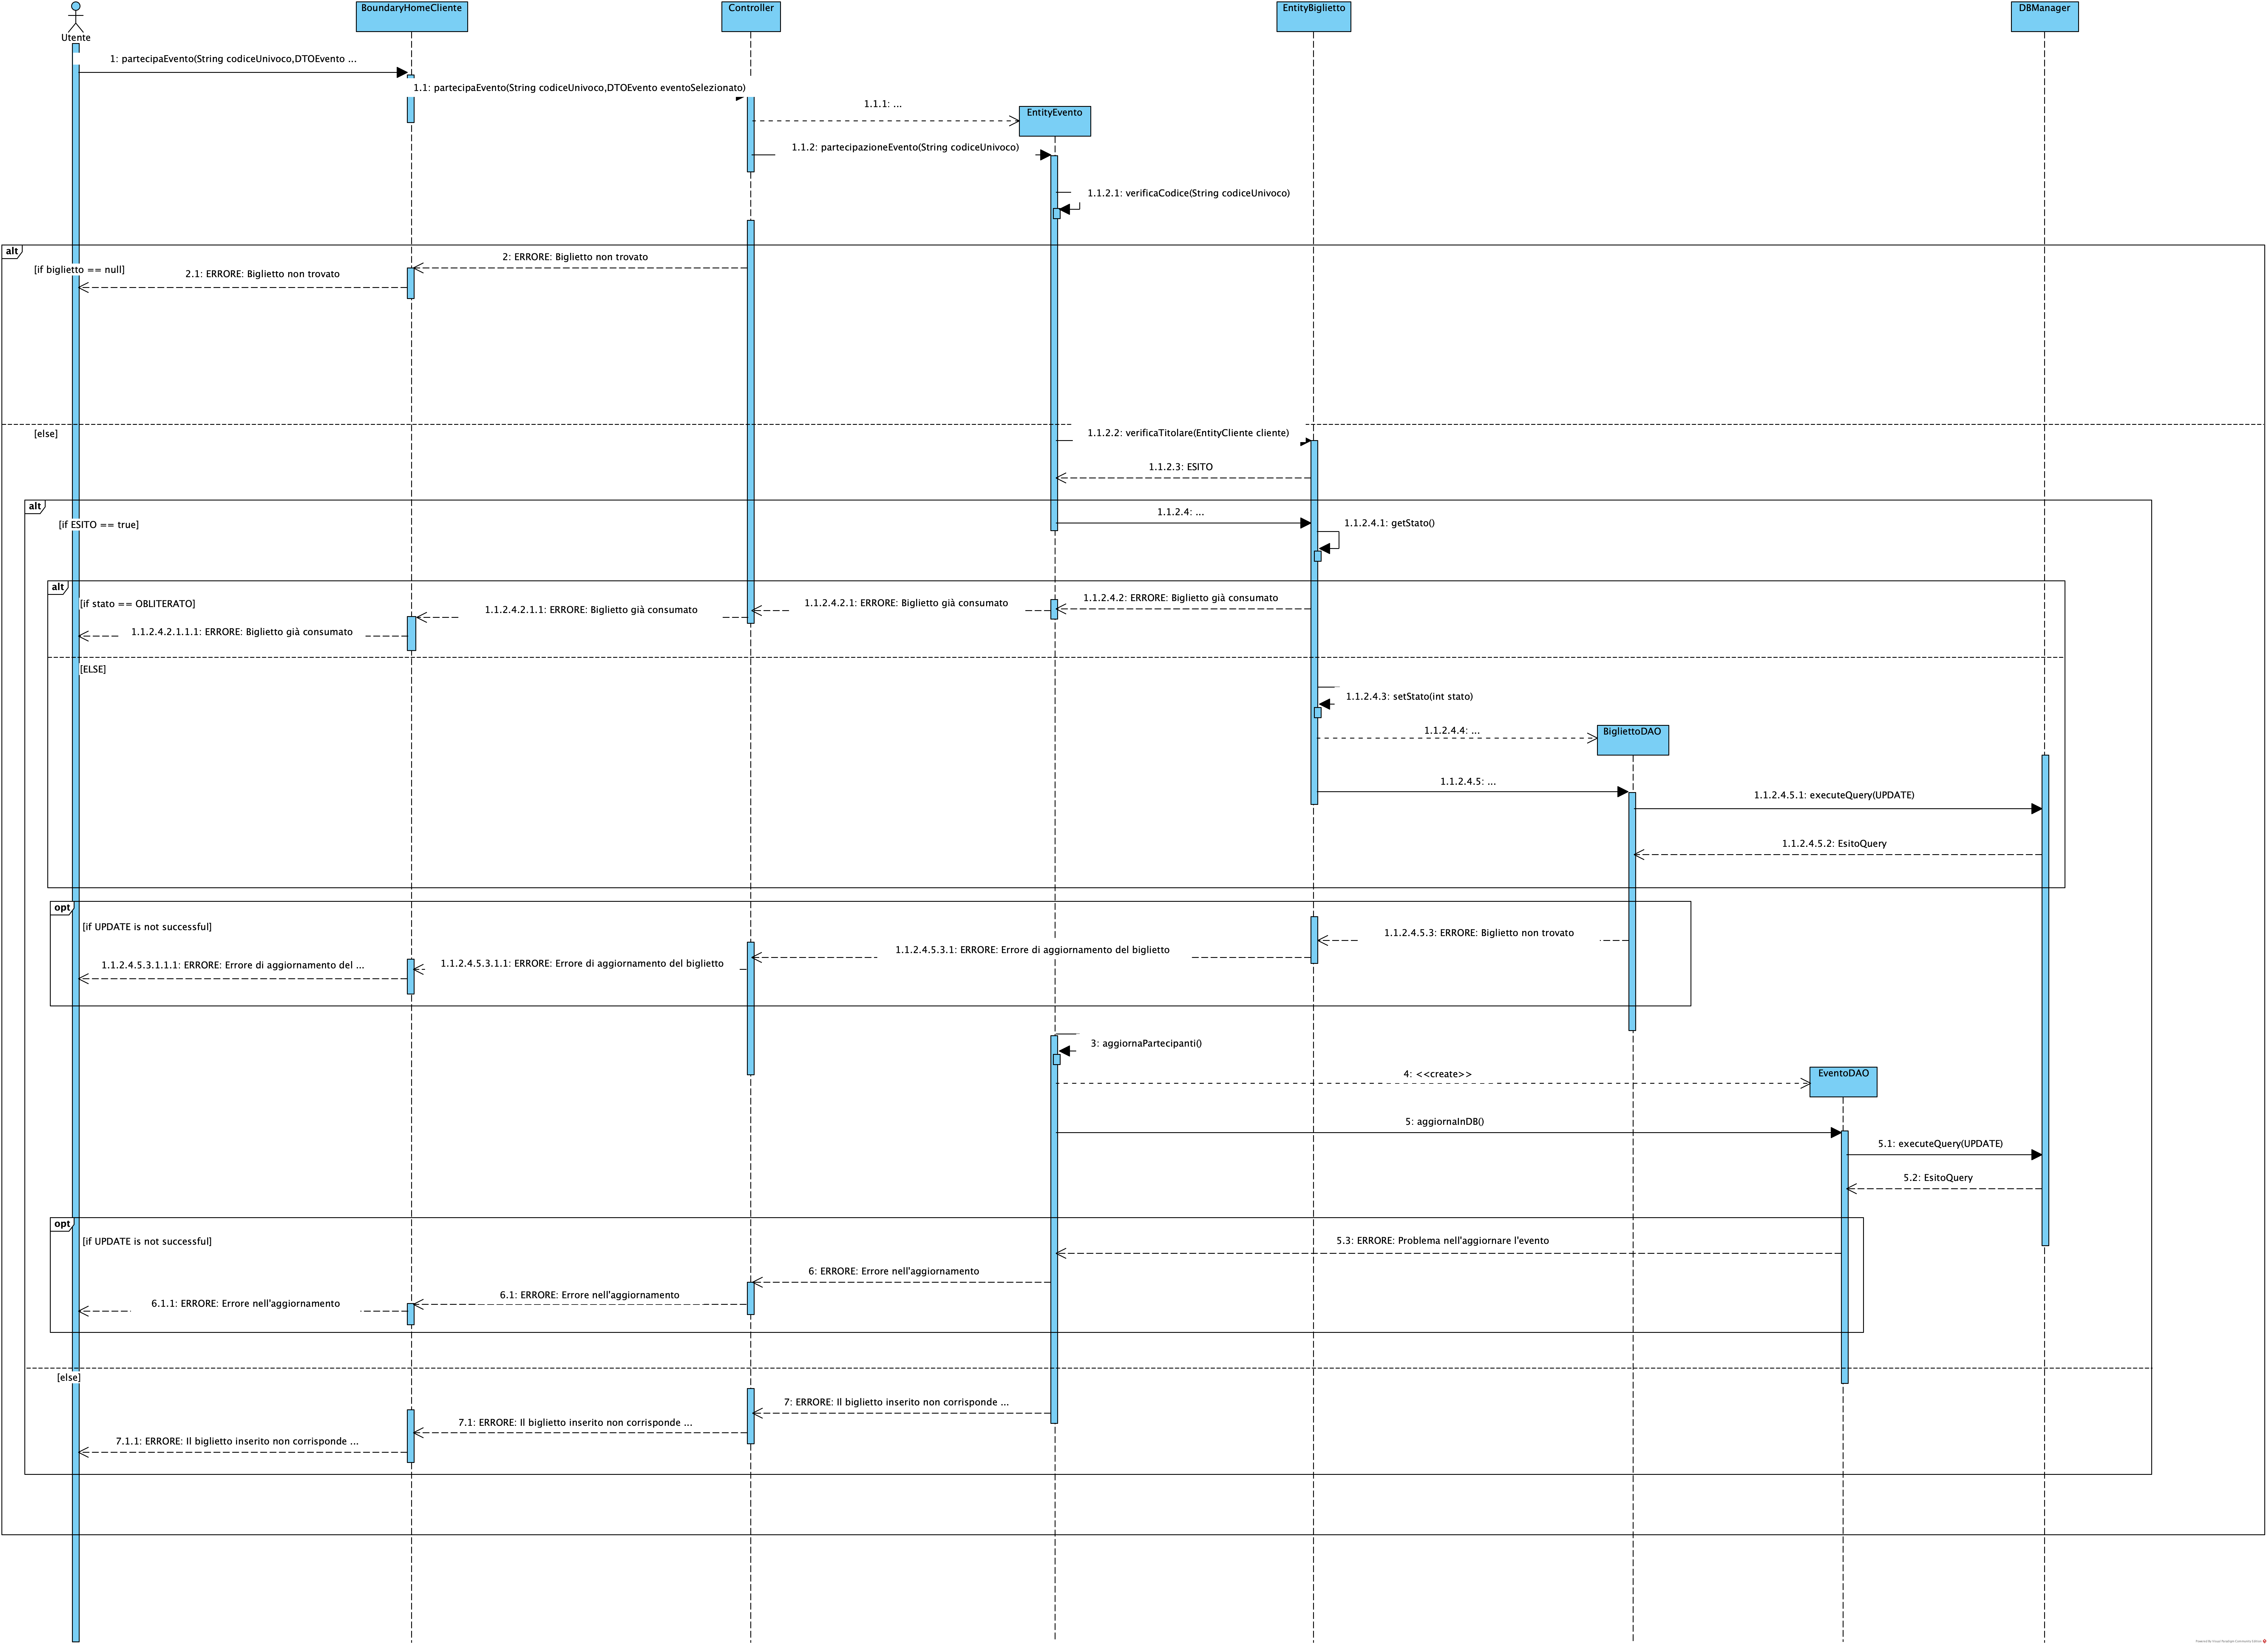
\includegraphics[width=\linewidth]{assets/SDProgettazione/PartecipazioneEventoProgettazione.png}
\caption{Sequence Diagram avanzato dello scenario \textit{PartecipazioneEvento} }
\end{figure}






